\documentclass[journal, a4paper]{IEEEtran}

% some very useful LaTeX packages include:

%\usepackage{cite}      % Written by Donald Arseneau
                        % V1.6 and later of IEEEtran pre-defines the format
                        % of the cite.sty package \cite{} output to follow
                        % that of IEEE. Loading the cite package will
                        % result in citation numbers being automatically
                        % sorted and properly "ranged". i.e.,
                        % [1], [9], [2], [7], [5], [6]
                        % (without using cite.sty)
                        % will become:
                        % [1], [2], [5]--[7], [9] (using cite.sty)
                        % cite.sty's \cite will automatically add leading
                        % space, if needed. Use cite.sty's noadjust option
                        % (cite.sty V3.8 and later) if you want to turn this
                        % off. cite.sty is already installed on most LaTeX
                        % systems. The latest version can be obtained at:
                        % http://www.ctan.org/tex-archive/macros/latex/contrib/supported/cite/

\usepackage{graphicx}   % Written by David Carlisle and Sebastian Rahtz
                        % Required if you want graphics, photos, etc.
                        % graphicx.sty is already installed on most LaTeX
                        % systems. The latest version and documentation can
                        % be obtained at:
                        % http://www.ctan.org/tex-archive/macros/latex/required/graphics/
                        % Another good source of documentation is "Using
                        % Imported Graphics in LaTeX2e" by Keith Reckdahl
                        % which can be found as esplatex.ps and epslatex.pdf
                        % at: http://www.ctan.org/tex-archive/info/

%\usepackage{psfrag}    % Written by Craig Barratt, Michael C. Grant,
                        % and David Carlisle
                        % This package allows you to substitute LaTeX
                        % commands for text in imported EPS graphic files.
                        % In this way, LaTeX symbols can be placed into
                        % graphics that have been generated by other
                        % applications. You must use latex->dvips->ps2pdf
                        % workflow (not direct pdf output from pdflatex) if
                        % you wish to use this capability because it works
                        % via some PostScript tricks. Alternatively, the
                        % graphics could be processed as separate files via
                        % psfrag and dvips, then converted to PDF for
                        % inclusion in the main file which uses pdflatex.
                        % Docs are in "The PSfrag System" by Michael C. Grant
                        % and David Carlisle. There is also some information
                        % about using psfrag in "Using Imported Graphics in
                        % LaTeX2e" by Keith Reckdahl which documents the
                        % graphicx package (see above). The psfrag package
                        % and documentation can be obtained at:
                        % http://www.ctan.org/tex-archive/macros/latex/contrib/supported/psfrag/

%\usepackage{subfigure} % Written by Steven Douglas Cochran
                        % This package makes it easy to put subfigures
                        % in your figures. i.e., "figure 1a and 1b"
                        % Docs are in "Using Imported Graphics in LaTeX2e"
                        % by Keith Reckdahl which also documents the graphicx
                        % package (see above). subfigure.sty is already
                        % installed on most LaTeX systems. The latest version
                        % and documentation can be obtained at:
                        % http://www.ctan.org/tex-archive/macros/latex/contrib/supported/subfigure/

\usepackage{url}        % Written by Donald Arseneau
                        % Provides better support for handling and breaking
                        % URLs. url.sty is already installed on most LaTeX
                        % systems. The latest version can be obtained at:
                        % http://www.ctan.org/tex-archive/macros/latex/contrib/other/misc/
                        % Read the url.sty source comments for usage information.

%\usepackage{stfloats}  % Written by Sigitas Tolusis
                        % Gives LaTeX2e the ability to do double column
                        % floats at the bottom of the page as well as the top.
                        % (e.g., "\begin{figure*}[!b]" is not normally
                        % possible in LaTeX2e). This is an invasive package
                        % which rewrites many portions of the LaTeX2e output
                        % routines. It may not work with other packages that
                        % modify the LaTeX2e output routine and/or with other
                        % versions of LaTeX. The latest version and
                        % documentation can be obtained at:
                        % http://www.ctan.org/tex-archive/macros/latex/contrib/supported/sttools/
                        % Documentation is contained in the stfloats.sty
                        % comments as well as in the presfull.pdf file.
                        % Do not use the stfloats baselinefloat ability as
                        % IEEE does not allow \baselineskip to stretch.
                        % Authors submitting work to the IEEE should note
                        % that IEEE rarely uses double column equations and
                        % that authors should try to avoid such use.
                        % Do not be tempted to use the cuted.sty or
                        % midfloat.sty package (by the same author) as IEEE
                        % does not format its papers in such ways.

\usepackage{amsmath}    % From the American Mathematical Society
                        % A popular package that provides many helpful commands
                        % for dealing with mathematics. Note that the AMSmath
                        % package sets \interdisplaylinepenalty to 10000 thus
                        % preventing page breaks from occurring within multiline
                        % equations. Use:
%\interdisplaylinepenalty=2500
                        % after loading amsmath to restore such page breaks
                        % as IEEEtran.cls normally does. amsmath.sty is already
                        % installed on most LaTeX systems. The latest version
                        % and documentation can be obtained at:
                        % http://www.ctan.org/tex-archive/macros/latex/required/amslatex/math/


\usepackage{url}
\usepackage{color,hyperref}
\definecolor{darkblue}{rgb}{0.0,0.0,0.55}
\hypersetup{colorlinks,breaklinks,
	linkcolor=darkblue,urlcolor=darkblue,
	anchorcolor=darkblue,citecolor=darkblue}
% Other popular packages for formatting tables and equations include:

%\usepackage{array}
% Frank Mittelbach's and David Carlisle's array.sty which improves the
% LaTeX2e array and tabular environments to provide better appearances and
% additional user controls. array.sty is already installed on most systems.
% The latest version and documentation can be obtained at:
% http://www.ctan.org/tex-archive/macros/latex/required/tools/

% V1.6 of IEEEtran contains the IEEEeqnarray family of commands that can
% be used to generate multiline equations as well as matrices, tables, etc.

% Also of notable interest:
% Scott Pakin's eqparbox package for creating (automatically sized) equal
% width boxes. Available:
% http://www.ctan.org/tex-archive/macros/latex/contrib/supported/eqparbox/

% *** Do not adjust lengths that control margins, column widths, etc. ***
% *** Do not use packages that alter fonts (such as pslatex).         ***
% There should be no need to do such things with IEEEtran.cls V1.6 and later.


% Your document starts here!
\begin{document}

% Define document title and author
	\title{MLANN; Maximum Likelihood Approximate Nearest Neighbor in Real-time Image Recognition}
	\author{\textsc{Ali Gholami\\ Department of Computer Engineering \& Information Technology\\ Amirkabir University of Technology}\\\textit{\url{https://aligholamee.github.io}\\\url{aligholami7596@gmail.com}}
	\thanks{Advisor: Professor Mohammad Rahmati}}
	\markboth{Statistical Pattern Recognition Final Project -- Week 1 -- April 14, 2018}{}
	\maketitle

% Write abstract here
\begin{abstract}
	In this report, a brief overview of the \textit{OpenFace} framework and the method behind it; \textit{FaceNet} is reviewed for the task of \textit{Image Recognition}.
\end{abstract}

% Each section begins with a \section{title} command
\section{Introduction}
	% \PARstart{}{} creates a tall first letter for this first paragraph
	\PARstart{A}{n} evolutionary paper \cite{HOP96} caused the \textit{Image Recognition} task to be more \textbf{accurate} and much more suitable for devices with lower \textbf{computational} power such as mobile devices. The mentioned paper has been implemented elaborately in the \textit{OpenFace} framework. The method is reviewed to gain a better understanding of how \textit{Image Recognition} methods can be implemented in practice.

% Main Part
\section{FaceNet Paper Goals}
	This paper supports the following three main goals for the task of \textit{Image Recognition}:\\
	\begin{itemize}
		\item Face Verification -- Is this the same person?
		\item Face Recognition -- Who is this person?
		\item Face Clustering -- Find common people among these faces?
	\end{itemize}

\section{The IDEA}
	The idea is that, we can learn Euclidean embedding per image using \textit{CNN} and the network is trained such that the squared L2 distances in the embedding space directly correspond to \textbf{face similarity}. 	The mentioned distance of two images illustrates whether two images are identical or not. In more details, a distance of $0.0$ illustrates the \textit{identity} of two images and a distance of $4.0$ shows that two images are completely in a \textit{opposite spectrum}. According to the results, a threshold of $1.1$ can correctly classify the images. Thus; if the distance of two images is less than $1.1$ it is representing the same person, otherwise they are different.

	% This is how you include a eps figure in your document. LaTeX only accepts EPS or TIFF files.
	\begin{figure}[!hbt]
		% Center the figure.
		\begin{center}
		% Include the eps file, scale it such that it's width equals the column width. You can also put width=8cm for example...
		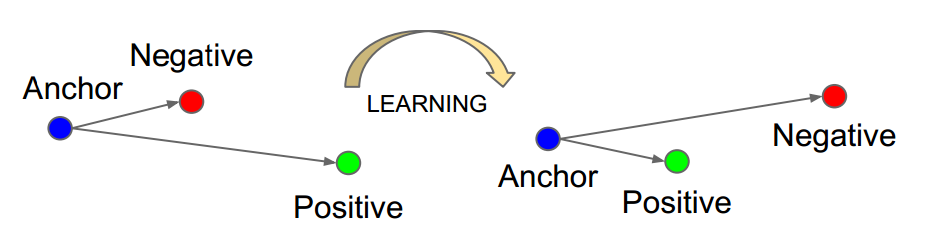
\includegraphics[width=\columnwidth]{distant_satellites.PNG}
		% Create a subtitle for the figure.
		\caption{The Triplet Loss minimizes the distance between an anchor and a positive, both of which have the same identity, and
			maximizes the distance between the anchor and a negative of a
			different identity.}
		% Define the label of the figure. It's good to use 'fig:title', so you know that the label belongs to a figure.
		\label{fig:tf_plot}
		\end{center}
	\end{figure}

\section{FaceNet's Method}
In order to reach the given idea, we have to consider using three images in every step of training:
\begin{enumerate}
	\item \textbf{Anchor} image -- The \textbf{actual} image we are learning the parameters with.
	\item \textbf{Positive} image -- The image that is representing the \textbf{same} person as in the Anchor image.
	\item \textbf{Negative} image -- The image that is representing a completely \textbf{different} person.
\end{enumerate}
We want to \textit{minimize} the distance between the \textit{Anchor} image and the \textit{Positive} image. Also, we want the distance between the \textit{Anchor} image and the \textit{Negative} image to be \textit{maximized}. Let $f(x)$ denote the embedding of image $x$ into a $d$ dimensional feature space $R^d$.  The given method can be written as:
$$
	||f(A) - f(P) ||^2 \leq ||f(A) - f(N) ||^2
$$
note that we have used the \textit{L2} distance. As always, we have to propose a \textit{loss} function. The loss function for the given formal representation is:
$$
	L(x_i^a,\ x_i^p,\ x_i^n) = \sum_{i = 0}^{N}[||f(x_i^a) - f(x_i^p)||^2 - ||f(x_i^a) - f(x_i^n)||^2 + \alpha]
$$
which  $x_i$ denotes the ith image in a set of $N$ images. $\alpha$ is a margin term that allows the faces for \textbf{one} identity to live on a \textbf{manifold}, while still enforcing the distance and discrimination from other identities.

% Now we need a bibliography:
\begin{thebibliography}{5}

	%Each item starts with a \bibitem{reference} command and the details thereafter.
	\bibitem{HOP96} % Transaction paper
	Schroff, Florian, Dmitry Kalenichenko, and James Philbin. "Facenet: A unified embedding for face recognition and clustering." Proceedings of the IEEE conference on computer vision and pattern recognition. 2015.

\end{thebibliography}

% Your document ends here!
\end{document}